\newthought{Intuitively}~any translative motion of a vortex should stem from an asymmetry of forces as in an imperfectly balanced gyroscope wobbling around and translating across a table.
The main effects that cause a quasi-geostrophic ocean eddy to translate laterally can be explained rel. easy heuristically:

\begin{marginfigure}
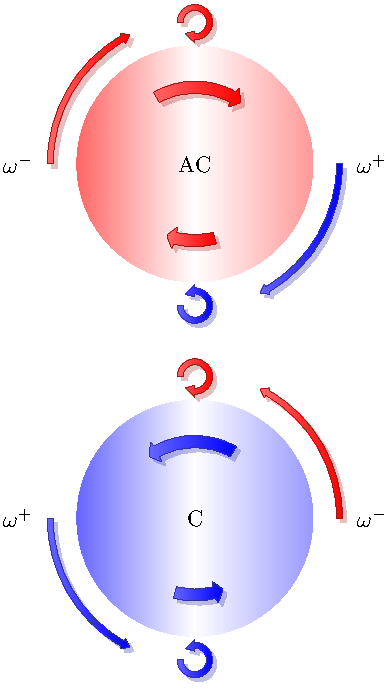
\includegraphics[width=1\textwidth]{eddyTikz}
\caption{Bottom [Top]: Northern hemisphere [anti]cyclone. Blue [red] color indicates presence/production of positive [negative] relative vorticity. Advection of adjacent water masses leads to a westward drift, irrespective of the eddy's sign (see~\cref{box:speed_planlift}). Inside, the discrepancy in swirl strength between north and south requires another (smaller) zonal drift term, which is eastward [westward] for [anti]cyclones. }
\label{fig:eddyTikz}
\end{marginfigure}

%\paragraph{Lateral Density Gradient}
%\label{paragraph:speed_dens}
%Consider a mean layer-thickness gradient $\dpr{h}{x}>0$ somewhere in the high northern latitudes and a geostrophic, positive density anomaly within that layer.
%In other words, a high-pressure vortex or an anti-cyclonic eddy with length scale $L\approx \mathrm{L_{R}}$.
%%Hence a vorticity budget dominated by advection of relative vorticity and vortex stretching.
%Next consider a parcel of water adjacent to the eddy's northern flank of initially zero relative vorticity that is being entrained by the eddy.
%As the clockwise rotating eddy advects the parcel towards its eastern side, the water-column comprising said fluid will be stretched vertically as it is advected towards larger depths. In order to maintain total vorticity a small new relative-vorticity term is introduced via term $C$ in \eqref{eq:vort7}.
%Since the vorticity budget is dominated by the planetary component, this new term has sign of $\f$ \ie \textbf{positive}.
%The opposite effect holds for a parcel advected towards the western side. Then, vortex \textit{squeezing} leads to a new \textbf{negative} relative-vorticity term.
%Hence water masses on both sides of the thickness gradient acquire rotation that slowly pushes the eddy in the direction $-\f\times \dpr{h}{x}$ (in this case south).
%Note  that since vorticity is dominated by the planetary component, the rotational sense of the eddy is irrelevant here. \Ie water columns stretched [squeezed], will always lead to new $\omega$ with sign of $\f$ [$-\f$].

%\paragraph{\textit{Planetary Lift}}
%\label{paragraph:speed_planlift}
%Assume now that $\beta L$ be comparable or larger even than $\f + \omega$ from the previous example.
%Then, independent of layer-thickness, all fluid adjacent to the eddy on its northern and southern flanks will be transported meridionally, thereby be tilted with respect to $\vec{\Omega}$ and hence acquire relative vorticity to compensate.
%All fluid transported north [south] will balance the increase in planetary vorticity with a decrease [increase] in relative vorticity. This is again independent of the eddy's sense and in this case also independent of hemisphere since $\dpr{f}{y}=\beta>0$ for all latitudes.
%The result is that small negative vortices to the northern and small positive vortices to the southern flank of eddies will push them west.

%\paragraph{Eddy-Internal $\beta$-Effect}
%\label{paragraph:speed_beta}
%In the later case clearly particles within the vortex undergo a change in planetary vorticity as well.
%Or from a different point of view, since $U \sim \grad p/f  $, and noting that the pressure gradient is the driving force here and hence fix at first approximation, particles drifting north will decelerate and those drifting south will accelerate.
%In order to maintain mass continuity, the center of volume will be shifted west for an anti-cyclone and east for a cyclone.
%Another way to look at it is to note that the only way for the discrepancy in Coriolis acceleration north and south, whilst maintaining constant eddy-relative particle speed, is to superimpose a zonal drift velocity so that net particle velocities achieve symmetric Coriolis acceleration.

\begin{driftspeed}[Lateral Density Gradient]
\label{box:speed_dens}
Consider a mean layer-thickness gradient $\dpr{h}{x}>0$ somewhere in the high northern latitudes and a geostrophic, positive density anomaly within that layer.
In other words, a high-pressure vortex or an anti-cyclonic eddy with length scale $L\approx \mathrm{L_{R}}$.
%Hence a vorticity budget dominated by advection of relative vorticity and vortex stretching.
Next consider a parcel of water adjacent to the eddy's northern flank of initially zero relative vorticity that is being entrained by the eddy.
As the clockwise rotating eddy advects the parcel towards its eastern side, the water-column comprising said fluid will be stretched vertically as it is advected towards larger depths. In order to maintain total vorticity a small new relative-vorticity term is introduced via term $C$ in \eqref{eq:vort7}.
Since the vorticity budget is dominated by the planetary component, this new term has sign of $\f$ \ie \textbf{positive}.
The opposite effect holds for a parcel advected towards the western side. Then, vortex \textit{squeezing} leads to a new \textbf{negative} relative-vorticity term.
Hence water masses on both sides of the thickness gradient acquire rotation that slowly pushes the eddy in the direction $-\f\times \dpr{h}{x}$ (in this case south).
Note  that since vorticity is dominated by the planetary component, the rotational sense of the eddy is irrelevant here. \Ie water columns stretched [squeezed], will always lead to new $\omega$ with sign of $\f$ [$-\f$].
\end{driftspeed}

\begin{marginfigure}
\includegraphics[]{SSHB.pdf}
  \caption{top: Stommel's equation $\mathrm{F}_{bottom}-\mathrm{F}_{surface}= -V\beta$ with constant eddy viscosity. bottom: \POP~eddy-resolving model snapshot with \SSH~mean of one year subtracted. }
  \label{fig:SSHB}
\end{marginfigure}

\begin{driftspeed}[Planetary Lift]
\label{box:speed_planlift}
Assume now that $\dfdy L$ be comparable or larger even than $\f + \omega$ from the previous example.
Then, independent of layer-thickness, all fluid adjacent to the eddy on its northern and southern flanks will be transported meridionally, thereby be tilted with respect to $\vec{\Omega}$ and hence acquire relative vorticity to compensate.
All fluid transported north [south] will balance the increase in planetary vorticity with a decrease [increase] in relative vorticity. This is again independent of the eddy's sense and in this case also independent of hemisphere since $\dpr{f}{y}=\dfdy>0$ for all latitudes.
The result is that small negative vortices to the northern and small positive vortices to the southern flank of eddies will push them west.
\end{driftspeed}

\begin{driftspeed}[Eddy-Internal $\dfdy$-Effect]
\label{box:speed_beta}
In the later case clearly particles within the vortex undergo a change in planetary vorticity as well.
Or from a different point of view, since $U \sim \grad p/f  $, and noting that the pressure gradient is the driving force here and hence fix at first approximation, particles drifting north will decelerate and those drifting south will accelerate.
In order to maintain mass continuity, the center of volume will be shifted west for an anti-cyclone and east for a cyclone.
Another way to look at it is to note that the only way for the discrepancy in Coriolis acceleration north and south, whilst maintaining constant eddy-relative particle speed, is to superimpose a zonal drift velocity so that net particle velocities achieve symmetric Coriolis acceleration.
\end{driftspeed}


%(see \cref{box:speed_dens})
